% Fig 2.6 — The three retrieval metrics on one worked example.
%
% GENERATED FILE — do not edit by hand.
% Source: thesis_figures/gen_fig_2_6_metrics.py   (regenerate, do not patch)
%
% Why this figure exists: NDCG@10 is the headline number of the whole thesis, and
% §2.2.4 defines it with two equations and no intuition. One example covers all
% three metrics and shows WHY they disagree, which a definition list cannot do.
\documentclass[border=4pt]{standalone}
\usepackage{tikz}
\usepackage{amsmath}
% Shared TikZ style for thesis figures.
% Each fig_*.tex \input{} this file after \usepackage{tikz}.
% Defines a muted, examiner-friendly color palette and semantic box styles.

\usepackage{xcolor}
\usepackage{fontawesome5}
\usetikzlibrary{positioning, arrows.meta, shapes.geometric, calc, fit, backgrounds}

% ─── Palette ───────────────────────────────────────────────────────────
% Each role has a stroke color (dark) and a fill color (very light).
% Designed to be grayscale-safe — lightness differs enough that B&W printing
% still preserves the distinction.

\definecolor{thQueryS}{HTML}{4A6FA5}    \definecolor{thQueryF}{HTML}{E8EEF6}   % query / input
\definecolor{thLLMS}{HTML}{6D4A8F}      \definecolor{thLLMF}{HTML}{ECE5F2}     % LLM / generation
\definecolor{thRetS}{HTML}{3D7A4F}      \definecolor{thRetF}{HTML}{E4EFE7}     % retriever
\definecolor{thDataS}{HTML}{6A6A6A}     \definecolor{thDataF}{HTML}{F1F1F1}    % corpus / data
\definecolor{thFusionS}{HTML}{A05A30}   \definecolor{thFusionF}{HTML}{F4E8DF}  % fusion
\definecolor{thOutS}{HTML}{1F6F8A}      \definecolor{thOutF}{HTML}{DEEAEF}     % output / final
\definecolor{thHiS}{HTML}{0D4D63}       \definecolor{thHiF}{HTML}{C8D9DF}      % highlighted (our contribution)
\definecolor{thMuted}{HTML}{5C5C5C}

% ─── Box styles ────────────────────────────────────────────────────────
% Usage in tikzpicture options:  query/.style={thQuery}, llm/.style={thLLM}, ...
% Or directly on nodes:          \node[thLLM] (m) {...};
\tikzset{
  thBase/.style={rectangle, draw, rounded corners=2pt,
                 minimum width=28mm, minimum height=10mm,
                 align=center, font=\small, line width=0.6pt,
                 inner sep=4pt},
  thQuery/.style={thBase, draw=thQueryS, fill=thQueryF},
  thLLM/.style={thBase, draw=thLLMS, fill=thLLMF},
  thRet/.style={thBase, draw=thRetS, fill=thRetF},
  thData/.style={cylinder, shape border rotate=90, aspect=0.3, draw=thDataS, fill=thDataF,
                 minimum width=24mm, minimum height=12mm, align=center, font=\small, line width=0.6pt},
  thFusion/.style={thBase, draw=thFusionS, fill=thFusionF},
  thOut/.style={thBase, draw=thOutS, fill=thOutF},
  thHi/.style={thBase, draw=thHiS, fill=thHiF, line width=1pt},
  thArrow/.style={-{Stealth[length=2.5mm]}, line width=0.7pt, draw=thMuted},
  thLabel/.style={font=\footnotesize\itshape, color=thMuted},
  thStage/.style={font=\bfseries\footnotesize, color=thMuted},
}

% ─── Icon helpers ──────────────────────────────────────────────────────
% Tiny FontAwesome icons that can sit inside a node prefix.
% Usage:  \node[thQuery] {\thIconQuery~User query};
\newcommand{\thIconQuery}{\textcolor{thQueryS}{\faSearch}}
\newcommand{\thIconUser}{\textcolor{thQueryS}{\faUser}}
\newcommand{\thIconLLM}{\textcolor{thLLMS}{\faBrain}}
\newcommand{\thIconRet}{\textcolor{thRetS}{\faNetworkWired}}
\newcommand{\thIconCorpus}{\textcolor{thDataS}{\faDatabase}}
\newcommand{\thIconFusion}{\textcolor{thFusionS}{\faCodeBranch}}
\newcommand{\thIconOut}{\textcolor{thOutS}{\faFile}}
\newcommand{\thIconEval}{\textcolor{thOutS}{\faChartBar}}
\newcommand{\thIconStar}{\textcolor{thHiS}{\faStar}}
\newcommand{\thIconCog}{\textcolor{thMuted}{\faCog}}


\begin{document}
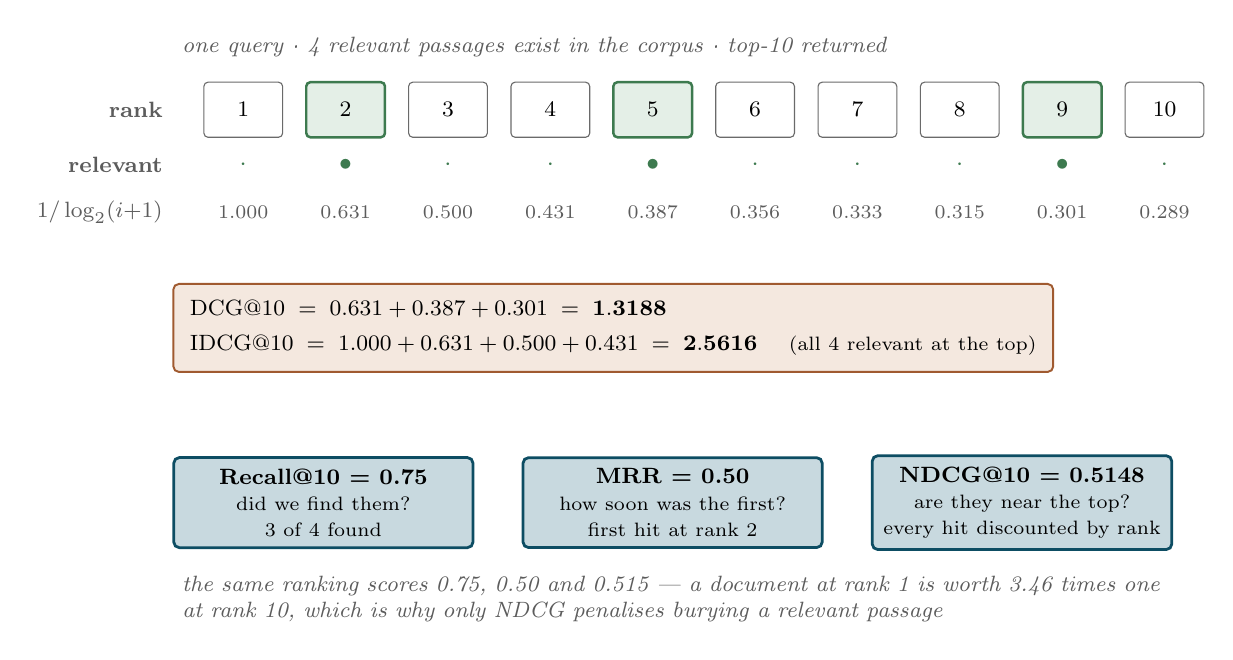
\begin{tikzpicture}[
    slot/.style={rectangle, draw=thDataS, fill=white, rounded corners=1.5pt,
                 minimum width=10mm, minimum height=7mm, font=\footnotesize},
    hit/.style={draw=thRetS, fill=thRetF, line width=0.9pt},
    relmark/.style={font=\small, color=thRetS},
    discval/.style={font=\scriptsize, color=thMuted},
    rowlab/.style={font=\footnotesize\bfseries, color=thMuted, anchor=east},
    calc/.style={rectangle, draw=thFusionS, fill=thFusionF, rounded corners=2pt,
                 align=left, inner sep=6pt, font=\footnotesize, line width=0.7pt},
    verdict/.style={thBase, draw=thHiS, fill=thHiF, line width=1pt,
                    align=center, font=\footnotesize, minimum height=8mm}
]

  % ─── The ranked list ────────────────────────────────────────────────────
    \node[slot] (s1) at (0mm, 0) {1};
  \node[slot,hit] (s2) at (13mm, 0) {2};
  \node[slot] (s3) at (26mm, 0) {3};
  \node[slot] (s4) at (39mm, 0) {4};
  \node[slot,hit] (s5) at (52mm, 0) {5};
  \node[slot] (s6) at (65mm, 0) {6};
  \node[slot] (s7) at (78mm, 0) {7};
  \node[slot] (s8) at (91mm, 0) {8};
  \node[slot,hit] (s9) at (104mm, 0) {9};
  \node[slot] (s10) at (117mm, 0) {10};
    \node[relmark] at (0mm, -7mm) {$\cdot$};
  \node[relmark] at (13mm, -7mm) {$\bullet$};
  \node[relmark] at (26mm, -7mm) {$\cdot$};
  \node[relmark] at (39mm, -7mm) {$\cdot$};
  \node[relmark] at (52mm, -7mm) {$\bullet$};
  \node[relmark] at (65mm, -7mm) {$\cdot$};
  \node[relmark] at (78mm, -7mm) {$\cdot$};
  \node[relmark] at (91mm, -7mm) {$\cdot$};
  \node[relmark] at (104mm, -7mm) {$\bullet$};
  \node[relmark] at (117mm, -7mm) {$\cdot$};
    \node[discval] at (0mm, -13mm) {1.000};
  \node[discval] at (13mm, -13mm) {0.631};
  \node[discval] at (26mm, -13mm) {0.500};
  \node[discval] at (39mm, -13mm) {0.431};
  \node[discval] at (52mm, -13mm) {0.387};
  \node[discval] at (65mm, -13mm) {0.356};
  \node[discval] at (78mm, -13mm) {0.333};
  \node[discval] at (91mm, -13mm) {0.315};
  \node[discval] at (104mm, -13mm) {0.301};
  \node[discval] at (117mm, -13mm) {0.289};

  \node[rowlab] at (-9mm, 0)     {rank};
  \node[rowlab] at (-9mm, -7mm)  {relevant};
  \node[rowlab] at (-9mm, -13mm) {$1/\log_2(i{+}1)$};

  \node[thLabel, anchor=west] at (-9mm, 8mm)
    {one query · 4 relevant passages exist in the corpus · top-10 returned};

  % ─── The arithmetic ─────────────────────────────────────────────────────
  \node[calc, anchor=north west] at (-9mm, -22mm) (calcbox) {%
    $\text{DCG@}10 \;=\; 0.631 + 0.387 + 0.301
       \;=\; \mathbf{1.3188}$\\[3pt]
    $\text{IDCG@}10 \;=\; 1.000 + 0.631 + 0.500 + 0.431
       \;=\; \mathbf{2.5616}$
       \quad{\scriptsize(all 4 relevant at the top)}};

  % ─── The three verdicts ─────────────────────────────────────────────────
  \node[verdict, minimum width=38mm, anchor=north west] at (-9mm, -44mm) (v1)
    {\textbf{Recall@10 = 0.75}\\{\scriptsize did we find them?}\\
      {\scriptsize 3 of 4 found}};
  \node[verdict, minimum width=38mm, right=6mm of v1] (v2)
    {\textbf{MRR = 0.50}\\{\scriptsize how soon was the first?}\\
      {\scriptsize first hit at rank 2}};
  \node[verdict, minimum width=38mm, right=6mm of v2] (v3)
    {\textbf{NDCG@10 = 0.5148}\\{\scriptsize are they near the top?}\\
      {\scriptsize every hit discounted by rank}};

  \node[thLabel, anchor=north west, text width=125mm] at (-9mm, -58mm)
    {the same ranking scores 0.75, 0.50 and 0.515 --- a document at rank~1
     is worth 3.46 times one at rank~10, which is why only NDCG penalises
     burying a relevant passage};

\end{tikzpicture}
\end{document}
